\documentclass[main.tex]{subfiles}
\begin{document}

\chapter{Thesis context}
\thispagestyle{chapstyle}
\label{chap_systemModel}
\minitoc


In this chapter, we present the inputs of the PhD work imposed by the industrial context. We firstly describe in Section~\ref{sec_systemModel_appModel} an abstract model of the avionics applications under consideration. Secondly, we provide in Section~\ref{sec_systemModel_archiMppa} extensive details on the COTS target that was chosen by Airbus and motivate this choice. Finally, we clarify in Section~\ref{sec_systemModel_additionalConstraints} the constraints that must be met in an aerospace and industrial context, such as the need for WCET computability or the limitations on eligible mapping and scheduling techniques to keep certification costs low.


%In this chapter, we will detail the consequences of the aerospace and industrial context of this thesis. 
%In Section~\ref{sec_systemModel_appModel}, we provide a formal model of multi-periodic hard real-time parallel tasks representing the real avionics applications that we will consider throughout the thesis.
%We detail the architecture of the \mppalong and we analyze the reasons making it a good candidate for the design of future avionics computers in Section~\ref{sec_systemModel_archiMppa}.
%And finally, we will study in Section~\ref{sec_systemModel_additionalConstraints} the additional constraints that must be met in an aerospace and industrial context, such as the need for WCET computability or the limitations on eligible mapping and scheduling techniques to keep certification costs low.



\section{Application model}
\label{sec_systemModel_appModel}

In this section, we formalize the model of applications considered in the rest of the dissertation. This model is representative of existing control applications at Airbus and is thus imposed in the context of this thesis.
An application is a tuple $< \tau , \delta >$ where $\tau$ is a finite set of parallel tasks and $\delta$ is a finite set of data. 

\subsection{Parallel task model}
The set of tasks $\tau = \{ \tau_1 , \ldots , \tau_n \}$ is composed of several tasks $\tau_i = < S_i , P_i , T_i >$ with:
\begin{itemize}
    \item $S_i = \{ \tau_i^1 , \ldots , \tau_i^{n_i} \}$ is a finite set of $n_i$ sub-tasks. All sub-tasks are simultaneously activated at the activation of $\tau_i$ and share the same implicit deadline equal to the period of $\tau_i$. In addition, each sub-task is defined by $\tau_i^j = < C_i^j , M_i^j , I_i^j , O_i^j >$ with:
        \begin{itemize}
            \item $C_i^j$ the WCET of the sub-task;
            \item $M_i^j$ the memory footprint of the sub-task, including the size of code, static and read-only data;
            \item $I_i^j$ and $O_i^j$ respectively the input and output buffers~\footnote{The I/O buffers are used to represent the interactions with external components, i.e. transactions with the external DDR-SDRAM of the reception/emission of Ethernet frames.} in which $\tau_i^j$ reads or writes.
        \end{itemize}

    \item $P_i \subset S_i \times S_i$ is a set of ordered pairs of sub-tasks. $P_i$ represents precedence relations constraining the order of execution of the sub-tasks. More precisely, $(\tau_i^x , \tau_i^y) \in P_i$ indicates that $\tau_i^x$ must complete its execution before $\tau_i^y$ can start. The set of precedences is assumed to be cycle-free and so, $P_i$ can be represented with a \emph{Directed Acyclic Graph} (or \emph{DAG}).

    \item $T_i$ is the period of $\tau_i$. It also serves as implicit deadlines for all sub-tasks of $\tau_i$.
\end{itemize}

We define the \emph{Hyperperiod} of the taskset as $H = \underset{\forall i \in [1 , n]}{lcm} ( T_i )$ where $lcm$ is the \emph{least common multiple} function.

\subsection{Data exchanges and communications}
The data in $\delta = \{ \delta_1 , \ldots , \delta_m \}$ are produced and consumed by the sub-tasks of the application. More precisely, with $S = \underset{\tau_i \in \tau}{\bigcup} S_i$ the set of all sub-tasks in the application, each data $\delta_k$ is defined as a tuple $\delta_k = < m_k , prod , cons >$ where:
\begin{itemize}
    \item $m_k$ represents the size of the data;
    \item $prod : \delta \mapsto S$ associates each data to its unique producing sub-task;
    \item $cons : \delta \mapsto 2^S$ associates each data to the set of consuming sub-tasks.
\end{itemize}

Any two sub-tasks can exchange data, including pairs of sub-tasks that are not constrained by precedence relations. However, two sub-tasks constrained by precedence relations are always assumed to exchange data. Indeed, specifying a specific execution order of sub-tasks that do not communicate is usually not necessary in practice.

No assumption is made on the tasks periods. However, the model allows precedence relations only between sub-tasks of the same task, thus having the same period. Multi-rate precedences are not allowed. No such constraint is imposed on data. A data can be produced in a task and consumed in an other, even if the two tasks do not run at the same pace. The only assumption on such multi-rate data is that the consumed value is always the freshest one, that is, the one that was produced during the last activation of the producing sub-task. Doing so enables to bound the freshness of the consumed multi-rate data. The underlying assumption here is that the treatment made by a task of any multi-rate data is robust to its maximum production-to-consumption delay, that is equal to the period of the producing sub-task.


\begin{example}[Example of application model]
    \label{ex_systemModel_appModel}

    We consider an application composed of 2 tasks $\tau_1$ and $\tau_2$. $\tau_1$ is composed of 4 sub-tasks 
    $\{ \tau_1^1 , \ldots , \tau_1^4 \}$  and $\tau_2$ of 7 sub-tasks 
    $\{ \tau_2^1 , \ldots , \tau_2^7 \}$. The 11 sub-tasks exchange 15 data
    $\{ \delta_a , \ldots , \delta_o \}$, read from 1 input buffer $i_1$ and write in 1 output buffer $o_1$.
    The periods of $\tau_1$ and $\tau_2$ respectively are $T_1 = 24$ and $T_2 = 48$. 
    The precedence constraints between the sub-tasks are depicted in Figure~\ref{fig_all_appModelPrecs}.
    The production and consumption of data and I/O buffers are depicted in Figure~\ref{fig_all_appModelDataflow}.
    Table~\ref{table_stateOfTheArt_2_tableTasksetExample} provides the attributes of all sub-tasks (\emph{ck} stands for clock cycle).


    \begin{table}[]
        \centering
        \begin{tabular*}{0.8\linewidth}{@{\extracolsep{\fill}}  c c c c c }
            \hline
            Sub-task & $C_i^j$ (in ck) & $M_i^j$ (in KiB) & $I_i^j$ & $O_i^j$ \\
            \hline
            $\tau_1^1$ & 500    & 519  & $i_1$          & $\varnothing$  \\
            $\tau_1^2$ & 500    & 397  & $\varnothing$  & $\varnothing$  \\ 
            $\tau_1^3$ & 700    & 642  & $\varnothing$  & $\varnothing$  \\ 
            $\tau_1^4$ & 400    & 262  & $\varnothing$  & $\varnothing$  \\ 
            $\tau_2^1$ & 1,000  & 287  & $\varnothing$  & $\varnothing$  \\ 
            $\tau_2^2$ & 400    & 799  & $\varnothing$  & $\varnothing$  \\ 
            $\tau_2^3$ & 500    & 542  & $\varnothing$  & $\varnothing$  \\ 
            $\tau_2^4$ & 800    & 764  & $\varnothing$  & $\varnothing$  \\ 
            $\tau_2^5$ & 900    & 490  & $\varnothing$  & $\varnothing$  \\ 
            $\tau_2^6$ & 500    & 399  & $\varnothing$  & $o_1$  \\ 
            $\tau_2^7$ & 600    & 12   & $\varnothing$  & $\varnothing$  \\ 
            \hline
        \end{tabular*}
        \caption{Example of sub-tasks parameters}
        \label{table_stateOfTheArt_2_tableTasksetExample}
    \end{table}

    \begin{figure}
        \centering
        \begin{subfigure}[b]{0.49\linewidth}
            \centering
            
\begin{tikzpicture}
    \node[draw, label={$\tau_1$}, thick] (T_A) at(0,0) {
        \begin{tikzpicture}
            \node[circle, draw, thick, inner sep=0pt, minimum width=1cm] (t1) at (0,0) {$\tau_1^1$};
            \node[circle, draw, thick, inner sep=0pt, minimum width=1cm] (t2) at (-0.7,-1.4) {$\tau_1^2$};
            \node[circle, draw, thick, inner sep=0pt, minimum width=1cm] (t3) at (0.7,-1.4) {$\tau_1^3$};
            \node[circle, draw, thick, inner sep=0pt, minimum width=1cm] (t4) at (0,-2.8) {$\tau_1^4$};
            \draw[>=latex,thick,->] (t1)--(t2);
            \draw[>=latex,thick,->] (t1)--(t3);
            \draw[>=latex,thick,->] (t2)--(t4);
            \draw[>=latex,thick,->] (t3)--(t4);
        \end{tikzpicture}
    };
    \node[draw, label={$\tau_2$}, thick] (T_B) at (3.5,0) {
        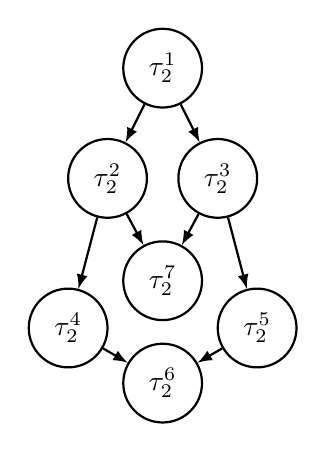
\begin{tikzpicture}
            % SEQ 1
            \node[circle, draw, thick, inner sep=0pt, minimum width=1cm] (t5) at (0,0) {$\tau_2^1$};
            \node[circle, draw, thick, inner sep=0pt, minimum width=1cm] (t6) at (-0.7,-1.4) {$\tau_2^2$};
            \node[circle, draw, thick, inner sep=0pt, minimum width=1cm] (t7) at (0.7,-1.4) {$\tau_2^3$};
            % SEQ 2
                \node[circle, draw, thick, inner sep=0pt, minimum width=1cm] (t8) at (-1.2,-3.3) {$\tau_2^4$};
            \node[circle, draw, thick, inner sep=0pt, minimum width=1cm] (t9) at (1.2,-3.3) {$\tau_2^5$};
            \node[circle, draw, thick, inner sep=0pt, minimum width=1cm] (t10) at (0,-4) {$\tau_2^6$};
            % SEQ 3
            \node[circle, draw, thick, inner sep=0pt, minimum width=1cm] (t11) at (0,-2.7) {$\tau_2^7$};
    
            % SEQ 1
            \draw[>=latex, thick,->] (t5)--(t6);
            \draw[>=latex, thick,->] (t5)--(t7);
            % SEQ 2
            \draw[>=latex, thick,->] (t8)--(t10);
            \draw[>=latex, thick,->] (t9)--(t10);
    
            % SEQ 1 -> SEQ 2
            \draw[>=latex, thick,->] (t6)--(t8);
            \draw[>=latex, thick,->] (t7)--(t9);
            % SEQ 1 -> SEQ 3
            \draw[>=latex, thick,->] (t6)--(t11);
            \draw[>=latex, thick,->] (t7)--(t11);
        \end{tikzpicture}
    };
\end{tikzpicture}

            \caption{Precedence constraints}
            \label{fig_all_appModelPrecs}
        \end{subfigure}
        \begin{subfigure}[b]{0.49\linewidth}
            \centering
            
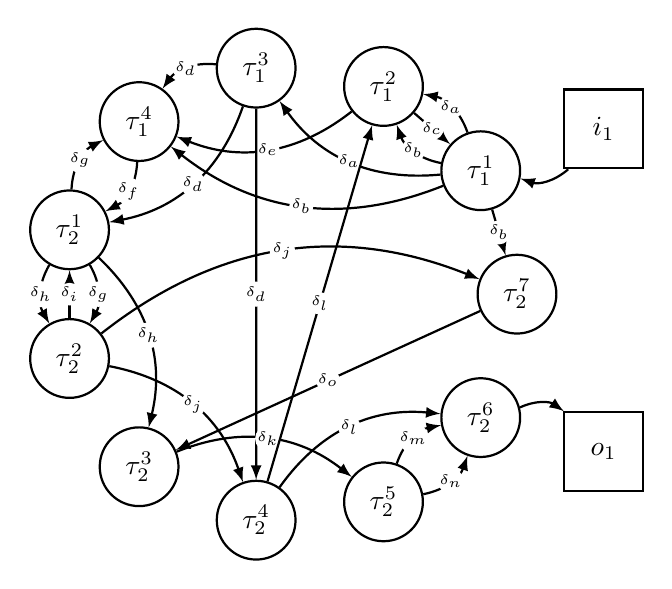
\begin{tikzpicture}
\tikzset{edgelabel/.style={fill=white, circle, inner sep=0pt, minimum size=0pt}}
\foreach \n in {1,2,...,4}{
    \node[ circle, draw, thick, inner sep=0pt, minimum width=1cm] (t\n)  at (\n*360/11: 2.9cm) {$\tau_1^{\n}$};
}
\foreach \n in {5,6,...,11}{
    \pgfmathsetmacro\result{\n - 4}
    \node[circle, draw, thick, inner sep=0pt, minimum width=1cm] (t\n)  at (\n*360/11: 2.9cm) {$\tau_2^{\pgfmathprintnumber{\result}}$};
}
\node[draw, thick, rectangle, inner sep=0pt, minimum size=1cm] (i1) at(4,2.1) {$i_1$};
\node[draw, thick, rectangle, inner sep=0pt, minimum size=1cm] (o1) at(4,-2.) {$o_1$};
\draw[-latex, thick, bend left] (i1) edge node[midway] {} (t1) ;
\draw[-latex, thick, bend left] (t10) edge node[midway] {} (o1) ;

\draw[-latex, thick, bend right] (t1) edge node[midway, edgelabel] {\tiny $\delta_a$} (t2) ;
\draw[-latex, thick, bend left] (t1) edge node[midway, edgelabel] {\tiny $\delta_b$} (t2);
\draw[-latex, thick, bend left] (t1) edge node[midway, edgelabel] {\tiny $\delta_a$} (t3);
\draw[-latex, thick, bend left] (t1) edge node[midway, edgelabel] {\tiny $\delta_b$} (t4);
\draw[-latex, thick] (t1) -- node[midway, edgelabel] {\tiny $\delta_b$} (t11);

\draw[-latex, thick] (t2) -- node[midway, edgelabel] {\tiny $\delta_c$} (t1);
\draw[-latex, thick, bend left] (t2) edge node[midway, edgelabel] {\tiny $\delta_e$} (t4);

\draw[-latex, thick, bend left] (t3) edge node[midway, edgelabel] {\tiny $\delta_d$} (t5);
\draw[-latex, thick, bend right] (t3) edge node[midway, edgelabel] {\tiny $\delta_d$} (t4);
\draw[-latex, thick] (t3) -- node[midway, edgelabel] {\tiny $\delta_d$} (t8);

\draw[-latex, thick, bend left] (t4) edge node[midway, edgelabel] {\tiny $\delta_f$} (t5);

\draw[-latex, thick, bend left] (t5) edge node[midway, edgelabel] {\tiny $\delta_g$} (t4);
\draw[-latex, thick, bend left] (t5) edge node[midway, edgelabel] {\tiny $\delta_g$} (t6);
\draw[-latex, thick, bend right] (t5) edge node[midway, edgelabel] {\tiny $\delta_h$} (t6);
\draw[-latex, thick, bend left] (t5) edge node[midway, edgelabel] {\tiny $\delta_h$} (t7);

\draw[-latex, thick] (t6) -- node[midway, edgelabel] {\tiny $\delta_i$} (t5);
\draw[-latex, thick, bend left] (t6) edge node[midway, edgelabel] {\tiny $\delta_j$} (t8);
\draw[-latex, thick, bend left] (t6) edge node[midway, edgelabel] {\tiny $\delta_j$} (t11);

\draw[-latex, thick, bend left] (t7) edge node[midway, edgelabel] {\tiny $\delta_k$} (t9);

\draw[-latex, thick] (t8) -- node[midway, edgelabel] {\tiny $\delta_l$} (t2);
\draw[-latex, thick, bend left] (t8) edge node[midway, edgelabel] {\tiny $\delta_l$} (t10);

\draw[-latex, thick, bend left] (t9) edge node[midway, edgelabel] {\tiny $\delta_m$} (t10);
\draw[-latex, thick, bend right] (t9) edge node[midway, edgelabel] {\tiny $\delta_n$} (t10);

\draw[-latex, thick] (t11) -- node[midway, edgelabel] {\tiny $\delta_o$} (t7);

\end{tikzpicture}

            \caption{Data and I/O buffers}
            \label{fig_all_appModelDataflow}
        \end{subfigure}
        \caption{Example of application model}
        \label{fig_stateOfTheArt_2_appModelExample}
    \end{figure}
\end{example}






















\section{Architecture of the \mppalong}
\label{sec_systemModel_archiMppa}
%Since the focus of this thesis is to leverage the massively parallel computational power of many-core processors, we will investigate the scheduling possibilities on such architecures. We consider a NoC-based many-core processor architecture featuring a distributed memory similar to the \mppalong.

%As depicted in Figure~\ref{fig_stateOfTheArt_2_genericManyCore}, such architecure is composed of several \emph{tiles}, each of which features some processing cores and some local memory. Since each tile has its own addressing space, the modification of a data in a local memory is not systematically seen by cores of other tiles. In such architecture, the hardware does not enforce data coherency. The software is fully in charge of commiting data modifications to other tiles through explicit message passing. This represents a major difference with mono- and multi-core processors where coherency is either inherent to the architecure or fully hardware-supported and transparent to software designers. 

%Moreover, software can be executed only with code and data that is locally present in the tile's memories. In this context, the locality of code and data appears to require particular attention to achieve good performance. So, the mapping of code and data on such processors will strongly depend on the storage capacity of the tiles. Yet, such memories are usually orders of magnitude smaller than external RAM chips (2MiB per tile in the \mppalong against several GiB for the external RAM). So, applications that used to face no storage issues when placed in RAM on on mono- or multi-core processors now need to be treated in a different manner to account for these new memory limitations.

%\begin{figure}
%    \centering
%    \scalebox{0.7}{% For building the DRAM structure figure
% #1 x, #2 y, #3 no
\newcommand\noctile[3]{
    \draw (#1,#2) node[circle, draw, thick, minimum size=1cm] (r#3) {R};
    \draw (0.7 + #1, -0.7 + #2) node[rectangle, draw, thick, dashed, minimum size=1.2cm, anchor=north west] (t#3) {\emph{Tile}};
    \draw (r#3.-45) edge[thick, dashed] (t#3.135);
}

\begin{tikzpicture}[font={\fontsize{12pt}{12}\selectfont}]

\noctile{0}{0}{1}
\noctile{0}{3}{2}
\noctile{0}{6}{3}
\noctile{0}{9}{4}
\noctile{3}{0}{5}
\noctile{3}{3}{6}
\noctile{3}{6}{7}
\noctile{3}{9}{8}
\noctile{6}{0}{9}
\noctile{6}{3}{10}
\noctile{6}{6}{11}
\noctile{6}{9}{12}
\noctile{9}{0}{13}
\noctile{9}{3}{14}
\noctile{9}{6}{15}
\noctile{9}{9}{16}

\draw (r1.east) edge[thick] (r5.west);
\draw (r2.east) edge[thick] (r6.west);
\draw (r3.east) edge[thick] (r7.west);
\draw (r4.east) edge[thick] (r8.west);
\draw (r5.east) edge[thick] (r9.west);
\draw (r6.east) edge[thick] (r10.west);
\draw (r7.east) edge[thick] (r11.west);
\draw (r8.east) edge[thick] (r12.west);
\draw (r9.east) edge[thick] (r13.west);
\draw (r10.east) edge[thick] (r14.west);
\draw (r11.east) edge[thick] (r15.west);
\draw (r12.east) edge[thick] (r16.west);

\draw (r1.north) edge[thick] (r2.south);
\draw (r2.north) edge[thick] (r3.south);
\draw (r3.north) edge[thick] (r4.south);
\draw (r5.north) edge[thick] (r6.south);
\draw (r6.north) edge[thick] (r7.south);
\draw (r7.north) edge[thick] (r8.south);
\draw (r9.north) edge[thick] (r10.south);
\draw (r10.north) edge[thick] (r11.south);
\draw (r11.north) edge[thick] (r12.south);
\draw (r13.north) edge[thick] (r14.south);
\draw (r14.north) edge[thick] (r15.south);
\draw (r15.north) edge[thick] (r16.south);

\end{tikzpicture}
}
%    \caption{Generic many-core architecture}
%    \label{fig_stateOfTheArt_2_genericManyCore}
%\end{figure}

The \mppalong \cite{kalray_mppa} is a many-core processor featuring 288 cores on a single chip. It targets the market of real-time computing-intensive low-power applications thanks to good temporal properties and a high computational power versus energy consumption ratio. In the following sections, we provide extensive details on the second version of the \mppalong architecture named \emph{Bostan}.

\subsection{Overview}
The \mppalong is organized in 16 \emph{compute clusters} dedicated to run user code. Four additional \emph{I/O clusters} serve as interfaces for managing communications with out-of-chip components or functions such as DDR-SDRAM or Ethernet. As depicted in Figure~\ref{fig_execModel_MPPANoCtopology}, all the clusters are interconnected with a dual 2D-torus NoC enabling point-to-point communications with explicit message-passing. 

\begin{figure}
    \centering
    \scalebox{1.5}{\begin{picture}(210,210)
    \put(0,0){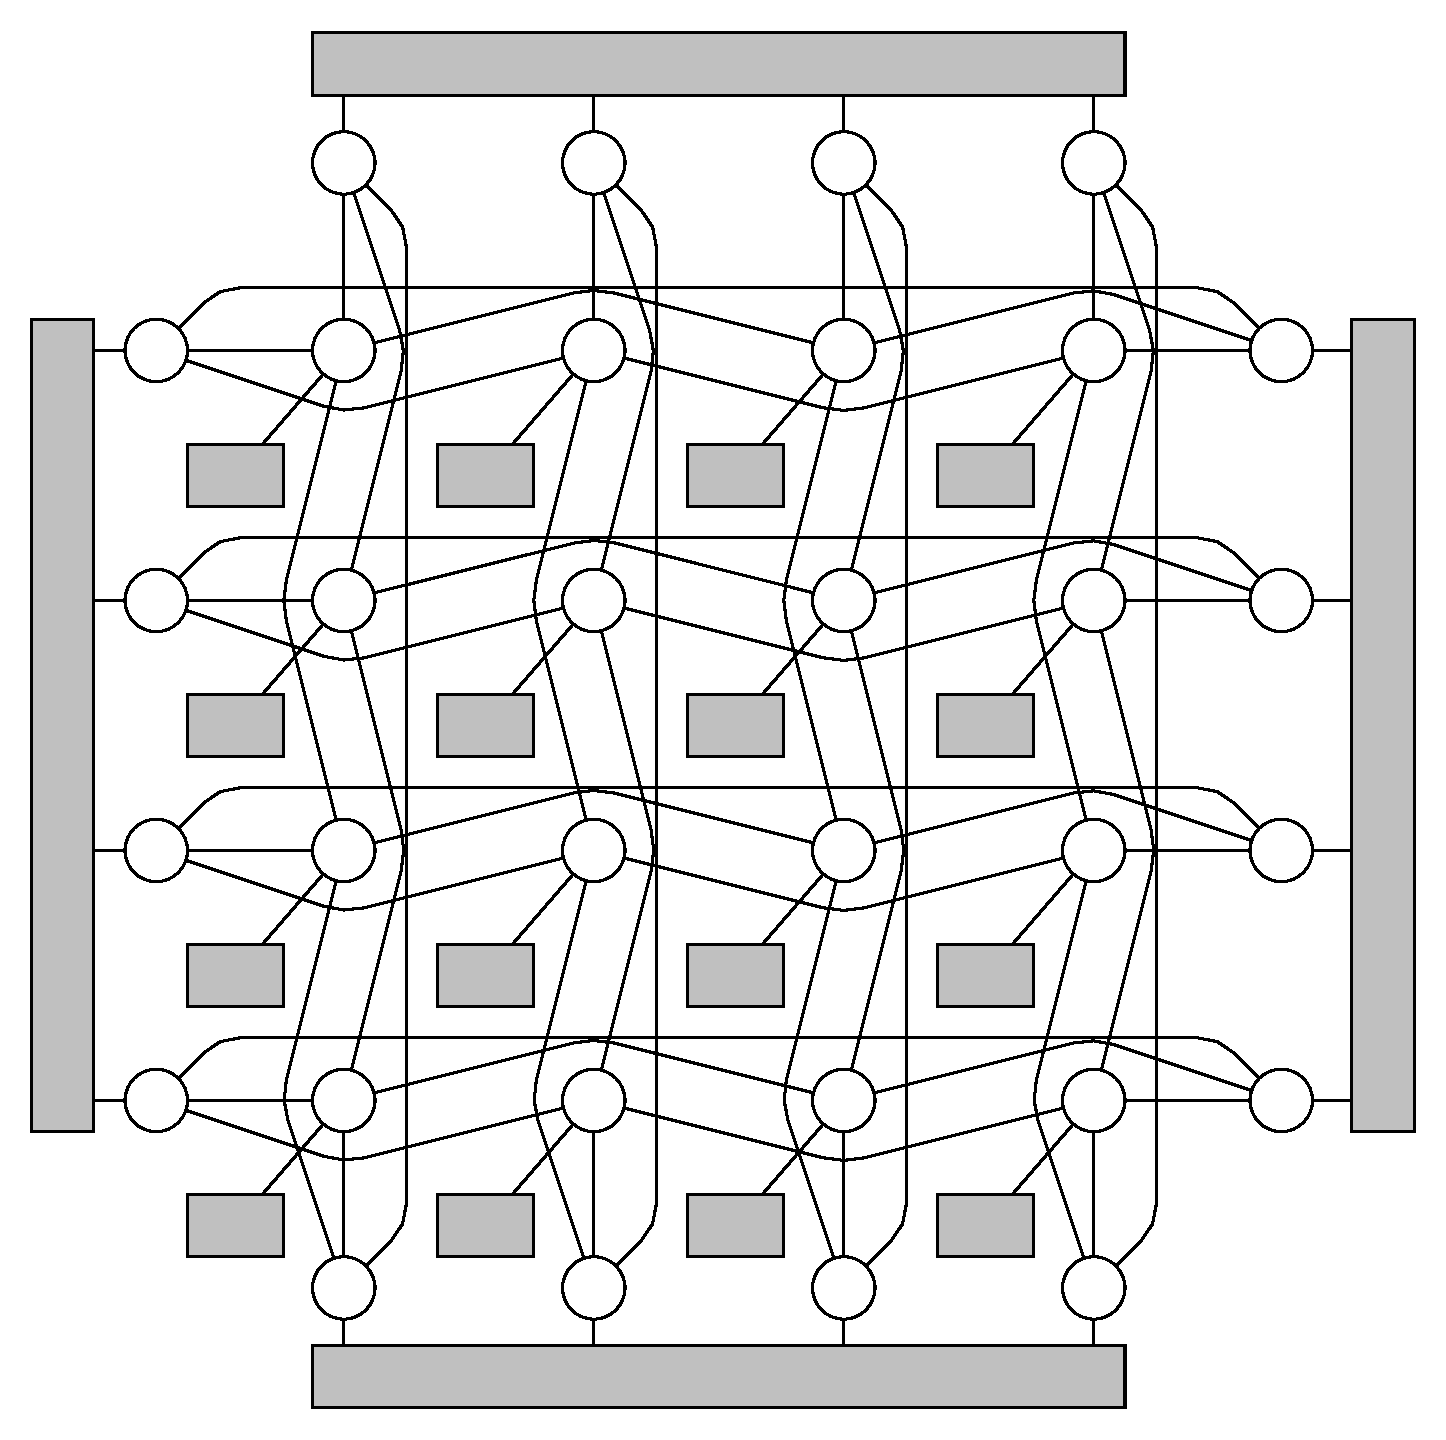
\includegraphics[width=210px]{imgs/pdf/all_MPPA_NoC_overview.pdf}}
    % I/O Tiles
    \put(75,7){\scriptsize \textit{South IO cluster}}
    \put(75,198){\scriptsize \textit{North IO cluster}}
    \put(6,74){\scriptsize \rotatebox{90}{\textit{West IO cluster}}}
    \put(199,133){\scriptsize \rotatebox{270}{\textit{East IO cluster}}}
    % Clusters 0-3
    \put(30, 139){\scriptsize $C_0$}
    \put(66, 139){\scriptsize $C_1$}
    \put(103,139){\scriptsize $C_2$}
    \put(139,139){\scriptsize $C_3$}
    % Clusters 4-7
    \put(30, 102){\scriptsize $C_4$}
    \put(66, 102){\scriptsize $C_5$}
    \put(103,102){\scriptsize $C_6$}
    \put(139,102){\scriptsize $C_7$}
    % Clusters 8-11
    \put(30, 66){\scriptsize $C_8$}
    \put(66, 66){\scriptsize $C_9$}
    \put(101,66){\scriptsize $C_{10}$}
    \put(137,66){\scriptsize $C_{11}$}
    % Clusters 12-15
    \put(28, 29){\scriptsize $C_{12}$}
    \put(64, 29){\scriptsize $C_{13}$}
    \put(101,29){\scriptsize $C_{14}$}
    \put(137,29){\scriptsize $C_{15}$}

    % Routers 0-3
    \put(47, 158){\scalebox{0.7}{\tiny $R_0$}}
    \put(83, 158){\scalebox{0.7}{\tiny $R_1$}}
    \put(120,158){\scalebox{0.7}{\tiny $R_2$}}
    \put(156,158){\scalebox{0.7}{\tiny $R_3$}}
    % Routers 4-7
    \put(47, 122){\scalebox{0.7}{\tiny $R_4$}}
    \put(83, 122){\scalebox{0.7}{\tiny $R_5$}}
    \put(120,122){\scalebox{0.7}{\tiny $R_6$}}
    \put(156,122){\scalebox{0.7}{\tiny $R_7$}}
    % Routers 8-11
    \put(47, 85){\scalebox{0.7}{\tiny $R_8$}}
    \put(83, 85){\scalebox{0.7}{\tiny $R_9$}}
    \put(119,85){\scalebox{0.7}{\tiny $R_{10}$}}
    \put(155,85){\scalebox{0.7}{\tiny $R_{11}$}}
    % Routers 12-15
    \put(46, 49){\scalebox{0.7}{\tiny $R_{12}$}}
    \put(82, 49){\scalebox{0.7}{\tiny $R_{13}$}}
    \put(119,49){\scalebox{0.7}{\tiny $R_{14}$}}
    \put(155,49){\scalebox{0.7}{\tiny $R_{15}$}}
    % Routers North
    \put(47, 186){\scalebox{0.7}{\tiny $R^n_0$}}
    \put(83, 186){\scalebox{0.7}{\tiny $R^n_1$}}
    \put(119,186){\scalebox{0.7}{\tiny $R^n_2$}}
    \put(156,186){\scalebox{0.7}{\tiny $R^n_3$}}
    % Routers South
    \put(47, 21){\scalebox{0.7}{\tiny $R^s_0$}}
    \put(83, 21){\scalebox{0.7}{\tiny $R^s_1$}}
    \put(119,21){\scalebox{0.7}{\tiny $R^s_2$}}
    \put(156,21){\scalebox{0.7}{\tiny $R^s_3$}}
    % Routers West
    \put(19,158){\scalebox{0.7}{\tiny $R^w_0$}}
    \put(19,122){\scalebox{0.7}{\tiny $R^w_1$}}
    \put(19, 85){\scalebox{0.7}{\tiny $R^w_2$}}
    \put(19, 49){\scalebox{0.7}{\tiny $R^w_3$}}
    % Routers East
    \put(183,158){\scalebox{0.7}{\tiny $R^e_0$}}
    \put(183,122){\scalebox{0.7}{\tiny $R^e_1$}}
    \put(183, 85){\scalebox{0.7}{\tiny $R^e_2$}}
    \put(183, 49){\scalebox{0.7}{\tiny $R^e_3$}}

    \end{picture}
}
    \caption{Architecture of the \mppalong}
    \label{fig_execModel_MPPANoCtopology}
\end{figure} 

\subsection{Compute clusters}
As depicted in Figure~\ref{fig_execModel_MPPAComputeCluster}, each compute cluster features:
\begin{itemize}
    \item 16 cores, denoted as the \emph{Processing Elements} (or \emph{PEs}), for executing user code;
    \item 1 additional core denoted as \emph{Resource Manager} or (\emph{RM}) in charge of managing and configuring the cluster's local resources;
    \item 1 \emph{Debug and Support Unit} (or \emph{DSU}) to ease programming and debugging with JTAG;
    \item 1 \emph{Direct Memory Access} (or \emph{DMA}) unit to automate data sending over the NoC;
    \item 2MiB of shared SRAM organized in 16 independent banks;
    \item 1 access to each NoC.
\end{itemize}



\begin{figure}
    \centering
    \scalebox{0.8}{
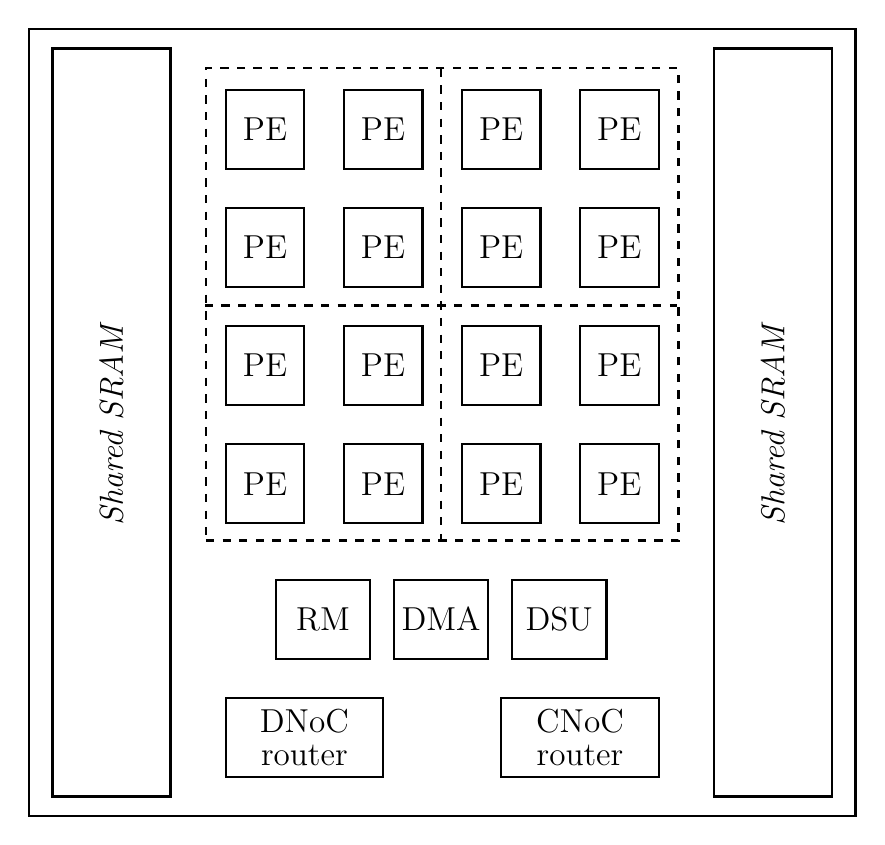
\begin{tikzpicture}[font={\fontsize{13pt}{12}\selectfont}]

    \node[rectangle, draw, color=black, thick, anchor=south west, minimum width=10.5cm, minimum height=10cm, inner sep=0pt] at (0,0.25) {};

    \node[rectangle, draw, color=black, thick, anchor=north west, minimum width=9.5cm, minimum height=1.5cm, inner sep=0pt, rotate=90] at (0.3,0.5) {\textit{Shared SRAM}};
    \node[rectangle, draw, color=black, thick, anchor=north west, minimum width=9.5cm, minimum height=1.5cm, inner sep=0pt, rotate=90] at (8.7,0.5) {\textit{Shared SRAM}};
    
%    \draw[color=black, thick, dashed] (0.25, 1.50) -- (1.75, 1.50); 
%    \draw[color=black, thick, dashed] (0.25, 2.75) -- (1.75, 2.75); 
%    \draw[color=black, thick, dashed] (0.25, 4) -- (1.75, 4); 
%    \draw[color=black, thick, dashed] (0.25, 5.25) -- (1.75, 5.25); 
%    \draw[color=black, thick, dashed] (0.25, 6.5) -- (1.75, 6.50); 
%    \draw[color=black, thick, dashed] (0.25, 7.75) -- (1.75, 7.75); 
%    \draw[color=black, thick, dashed] (0.25, 9) -- (1.75, 9); 


    \node[rectangle, draw, color=black, thick, anchor=north west, minimum width=1cm, minimum height=1cm, inner sep=0pt] at (2.5,9.5) {PE};
    \node[rectangle, draw, color=black, thick, anchor=north west, minimum width=1cm, minimum height=1cm, inner sep=0pt] at (4,  9.5) {PE};
    \node[rectangle, draw, color=black, thick, anchor=north west, minimum width=1cm, minimum height=1cm, inner sep=0pt] at (5.5,9.5) {PE};
    \node[rectangle, draw, color=black, thick, anchor=north west, minimum width=1cm, minimum height=1cm, inner sep=0pt] at (7,  9.5) {PE};

    \node[rectangle, draw, color=black, thick, anchor=north west, minimum width=1cm, minimum height=1cm, inner sep=0pt] at (2.5,8) {PE};
    \node[rectangle, draw, color=black, thick, anchor=north west, minimum width=1cm, minimum height=1cm, inner sep=0pt] at (4,  8) {PE};
    \node[rectangle, draw, color=black, thick, anchor=north west, minimum width=1cm, minimum height=1cm, inner sep=0pt] at (5.5,8) {PE};
    \node[rectangle, draw, color=black, thick, anchor=north west, minimum width=1cm, minimum height=1cm, inner sep=0pt] at (7,  8) {PE};
    
    \node[rectangle, draw, color=black, thick, anchor=north west, minimum width=1cm, minimum height=1cm, inner sep=0pt] at (2.5,6.5) {PE};
    \node[rectangle, draw, color=black, thick, anchor=north west, minimum width=1cm, minimum height=1cm, inner sep=0pt] at (4,  6.5) {PE};
    \node[rectangle, draw, color=black, thick, anchor=north west, minimum width=1cm, minimum height=1cm, inner sep=0pt] at (5.5,6.5) {PE};
    \node[rectangle, draw, color=black, thick, anchor=north west, minimum width=1cm, minimum height=1cm, inner sep=0pt] at (7,  6.5) {PE};

    \node[rectangle, draw, color=black, thick, anchor=north west, minimum width=1cm, minimum height=1cm, inner sep=0pt] at (2.5,5) {PE};
    \node[rectangle, draw, color=black, thick, anchor=north west, minimum width=1cm, minimum height=1cm, inner sep=0pt] at (4,  5) {PE};
    \node[rectangle, draw, color=black, thick, anchor=north west, minimum width=1cm, minimum height=1cm, inner sep=0pt] at (5.5,5) {PE};
    \node[rectangle, draw, color=black, thick, anchor=north west, minimum width=1cm, minimum height=1cm, inner sep=0pt] at (7,  5) {PE};
    
    \node[rectangle, draw, color=black, thick, anchor=south west, minimum width=6cm, minimum height=6cm, inner sep=0pt, dashed] at (2.25,3.75) {};
    \draw[color=black, thick, dashed] (2.25, 6.75) -- (8.25, 6.75); 
    \draw[color=black, thick, dashed] (5.25, 9.755) -- (5.25, 3.75); 
    
    \node[rectangle, draw, color=black, thick, anchor=south west, minimum width=2cm, minimum height=1cm, text width=1.5cm,  align=center,inner sep=0pt] at (2.5,  0.75) {DNoC\\ router};
    \node[rectangle, draw, color=black, thick, anchor=south west, minimum width=2cm, minimum height=1cm, text width=1.5cm,  align=center,inner sep=0pt] at (6,  0.75) {CNoC\\ router};

    \node[rectangle, draw, color=black, thick, anchor=south, minimum width=1.2cm, minimum height=1cm, inner sep=0pt] at (3.75,  2.25) {RM};
    \node[rectangle, draw, color=black, thick, anchor=south, minimum width=1.2cm, minimum height=1cm, inner sep=0pt] at (5.25,  2.25) {DMA};
    \node[rectangle, draw, color=black, thick, anchor=south, minimum width=1.2cm, minimum height=1cm, inner sep=0pt] at (6.75,  2.25) {DSU};
    
\end{tikzpicture}
}
    \caption{Architecture of compute clusters in the \mppalong}
    \label{fig_execModel_MPPAComputeCluster}
\end{figure}


\subsubsection{Shared SRAM}
The 2 MiB of SRAM in a compute cluster are organized in 16 independent banks. Two local masters of the cluster (among PEs, the RM, the DMA or the DSU) can target two different banks without suffering from interferences. Their memory access paths are not dependent. However, concurrent accesses from two masters targeting the same bank will be arbitrated with a hierarchical arbitration policy depicted in Figure~\ref{fig_execModel_MPPASMEMarbiter}.
\begin{figure}
    \centering
    \scalebox{0.8}{
% 1 : x; 2: y; 3: no; 4: tikz object name
\newcommand\smemarbpe[4]{
    \node[rectangle, draw, color=black, thick, anchor=south west, minimum width=1.2cm, minimum height=1cm, inner sep=0pt] (#4) at (#1, #2) {PE#3};
    \node[rectangle, draw, color=black, thick, anchor=south west, minimum width=0.8cm, minimum height=0.5cm, inner sep=0pt] (IC#4) at (#1 + 1.2, #2) {{\small I\$}};
    \node[rectangle, draw, color=black, thick, anchor=south west, minimum width=0.8cm, minimum height=0.5cm, inner sep=0pt] (DC#4) at (#1 + 1.2, #2 + 0.5) {{\small D\$}};
}

% 1 : x; 2: y; 3: tikz object name
\newcommand\smemRRarb[3]{
    \node[circle, draw, color=black, thick, minimum size=0.7cm, inner sep=0pt] (#3) at (#1, #2) {\textit{\scriptsize RR}};
    \draw[ultra thick, ->, >=latex] (#3.west) -- ([yshift=-0.6em]#3.west); 
}

\begin{tikzpicture}[font={\fontsize{12pt}{12}\selectfont}]


    \node[rectangle, draw, color=black, thick, anchor=south west, minimum width=2cm, minimum height=1cm, inner sep=0pt] (DMARx) at (0, 0) {DMA Rx};

    \node[rectangle, draw, color=black, thick, anchor=south west, minimum width=2cm, minimum height=1cm, inner sep=0pt] (DMATx) at (0, 1.5) {DMA Tx};
    \node[rectangle, draw, color=black, thick, anchor=south west, minimum width=2cm, minimum height=1cm, inner sep=0pt] (DSU) at (0, 3) {DSU};
    \node[rectangle, draw, color=black, thick, anchor=south west, minimum width=2cm, minimum height=1cm, inner sep=0pt] (RM) at (0, 4.5) {RM};
    \smemRRarb {4.5}{3.5}{rrRM}
    \draw[thick, ->, >=latex] (RM.east) -| (rrRM.north);
    \draw[thick, ->, >=latex] (DMATx.east) -| (rrRM.south);
    \draw[thick, ->, >=latex] (DSU.east) -- (rrRM.west);

    
    \smemarbpe{0}{6}{16}{pe16}
    \smemRRarb {3}{6.5}{rrpe16}
    \draw[thick, ->, >=latex] (ICpe16.east) -- (rrpe16.220);
    \draw[thick, ->, >=latex] (DCpe16.east) -- (rrpe16.135);
    \node at (1, 7.5) {{\Huge ...}};
    
    \smemarbpe{0}{8}{2}{pe2}
    \smemRRarb {3}{8.5}{rrpe2}
    \draw[thick, ->, >=latex] (ICpe2.east) -- (rrpe2.220);
    \draw[thick, ->, >=latex] (DCpe2.east) -- (rrpe2.135);
    
    \smemarbpe{0}{9.5}{1}{pe1}
    \smemRRarb {3}{10}{rrpe1}
    \draw[thick, ->, >=latex] (ICpe1.east) -- (rrpe1.220);
    \draw[thick, ->, >=latex] (DCpe1.east) -- (rrpe1.135);


    \smemRRarb {4.5}{8.5}{rrPEs}
    \draw[thick, ->, >=latex] (rrpe1.east) -| (rrPEs.north);
    \draw[thick, ->, >=latex] (rrpe2.east) -- (rrPEs.west);
    \draw[thick, ->, >=latex] (rrpe16.east) -| (rrPEs.south);
    
    \smemRRarb {6}{6}{rrFinal}
    \draw[thick, ->, >=latex] (rrPEs.east) -| (rrFinal.north);
    \draw[thick, ->, >=latex] (rrRM.east) -| (rrFinal.south);

    \node[circle, draw, color=black, fill=black, thick, minimum size=0.15cm, inner sep=0pt] (lpint) at (7, 6) {};
    \node[circle, draw, color=black, fill=black, thick, minimum size=0.15cm, inner sep=0pt] (hpint) at (7, 5.5) {};
    \node[circle, draw, color=black, fill=black, thick, minimum size=0.15cm, inner sep=0pt] (outint) at (7.7, 6) {};
    \node at (7.4, 6.4) {{\small Priority}};
    \draw[thick, ->, >=latex] (rrFinal.east) -- (lpint.west);
    \draw[thick, ->, >=latex] (DMARx.east) -| (hpint.south);
    \draw[thick] (hpint) -- (outint);
    
    \node[rectangle, draw, color=black, thick, anchor=south west, minimum width=2.5cm, minimum height=1cm, inner sep=0pt] (banki) at (9, 5.5) {\textit{Bank i}};
    \node[rectangle, draw, color=black, thick, anchor=south west, minimum width=2.5cm, minimum height=1cm, inner sep=0pt] at (9, 4) {\textit{Bank i+1}};
    \node[rectangle, draw, color=black, thick, anchor=south west, minimum width=2.5cm, minimum height=1cm, inner sep=0pt] at (9, 2.5) {\textit{Bank i+2}};
    \node[rectangle, draw, color=black, thick, anchor=south west, minimum width=2.5cm, minimum height=1cm, inner sep=0pt] at (9, 1) {\textit{Bank i+3}};
    \node[rectangle, draw, color=black, thick, anchor=south west, minimum width=2.5cm, minimum height=1cm, inner sep=0pt] at (9, 7) {\textit{Bank i-1}};
    \node[rectangle, draw, color=black, thick, anchor=south west, minimum width=2.5cm, minimum height=1cm, inner sep=0pt] at (9, 8.5) {\textit{Bank i-2}};
    \node[rectangle, draw, color=black, thick, anchor=south west, minimum width=2.5cm, minimum height=1cm, inner sep=0pt] at (9, 10) {\textit{Bank i-3}};

    \draw[thick, ->, >=latex] (outint.east) -- (banki.west);
    
\end{tikzpicture}
}
    \caption{Hierarchical SRAM arbiter of \mppalong}
    \label{fig_execModel_MPPASMEMarbiter}
\end{figure}

\begin{description}
    \item[Arbitration policy]
        Each local SRAM bank is accessible from 20 memory access paths: 16 serving the PEs (for both instruction and data caches), 1 for the RM, 1 for the DSU, 1 for the DMA when \emph{receiving} packets from the NoC and 1 for the DMA when \emph{emitting} packets. Each bank has a memory arbiter interleaving concurrent accesses from any of the 20 memory masters. PEs accesses are arbitrated in a Round-Robin fashion. Similarly, memory requests from the DSU, the RM and the DMA in emission are arbitrated in Round-Robin. The resulting accesses from this first level of arbitration enter another Round-Robin arbiter before eventually accessing the bank. The case of the received packets from the NoC is treated differently. The memory requests issued by the DMA when receiving packets have full priority over any other memory transactions to access any local SRAM bank. As a consequence, requests from PEs, the RM, the DMA in emission or the DSU are systematically stalled while the DMA writes the received data into memory. This is done to avoid congestion on the NoC.

    \item[Addressing modes]
        The local memory addressing can be configured in two modes at startup: \emph{interleaved} or \emph{blocked} addressing schemes. When in \emph{interleaved} mode, contiguous memory addresses jump from bank to bank every 64 bytes. This usually distributes the memory requests evenly over the 16 banks and provides good average performances without paying particular attention to the memory mapping. When in \emph{blocked} mode, contiguous memory areas are not shuffled among the banks and each bank can be addressed directly with a linear 128KiB address space.
\end{description}


\subsubsection{Intra-cluster communications}
\label{sssec_execModel_intraClusterComs}
The communication between local elements inside a compute cluster are essentially achieved with shared memory. The two exceptions lie in the PEs shared registers and the notification system signaling to the RM and PEs the occurrence of specific events.

\begin{description}
    \item[Cache coherency]
        Each core in a compute cluster features one private instruction cache of 8KiB and one private data cache of 8KiB. All caches use the \emph{Least Recently Used} (or \emph{LRU}) line replacement policy. Cache coherency is not enforced by any hardware mechanisms inside clusters and not between clusters either. Specific instructions are provided to achieve uncached memory accesses, to purge write-buffers and to invalidate caches.

    \item[Memory Management Units]
        Each core features a MMU capable of both virtual addressing and memory protection. \emph{Translation Lookaside Buffers} (or \emph{TLBs}) can be configured to enforce local caching policies (Write-Through or Bypass) on specific memory pages.


    \item[Events and shared registers]
        As depicted in Figure~\ref{fig_execModel_MPPAComputeCluster}, PEs are bundled in groups of four neighbors. In each group, PEs can send events to each others to achieve synchronization barriers. Moreover, the RM is capable of sending and receiving events to/from all PEs in the cluster.
        Each PE can also write directly to the 32 upper registers of its three neighbors. 
\end{description}


\subsubsection{Inter-cluster communications}
All the inter-cluster communications are achieved by explicit message passing or remote DMA through the NoC. The DMA in each cluster unloads the cores from the work of pushing or receiving data through the network interfaces. 

\begin{description}
    \item[Sending data]
        The DMA features a micro-engine capable of sending data through 8 \emph{Tx channels}. Each Tx channel can be configured independently. In particular, each Tx channel can be set-up with a specific route and specific traffic regulation parameters. Those configurations are done using memory-mapped registers that should be written by the RM. PEs may be allowed to write such configurations if and only if the RM previously updated permissions registers to explicitly allow it. 

        The micro-engine of the DMA can run up to 8 threads simultaneously. Each thread will push data through any of the 8 Tx channels. In particular, each thread executes instructions from a specific binary code resulting from the compilation of a \emph{micro-code} expressed in a light Kalray-specific assembly language. Threads can read parameters from memory-mapped registers that are written by the RM, or possibly the PEs if permission registers allow it. Those parameters can be used to pass the base address and the length of a buffer that shall be sent by the DMA for example.

    \item[Receiving data]
        The DMA features 256 \emph{Rx channels} that can be configured independently. Each Rx channel can be associated with a buffer of fixed length in the local SRAM. All the packets received through this channel will be written in this memory area. In addition, each Rx channel can be configured in a specific mode to notify the RM when an \emph{End of Transmission} (or \emph{EOT}) message has been received or when the total amount of data received overpassed a predefinite trigger for example.
\end{description}

\subsubsection{Debug and Support Unit}
Each cluster has a local DSU which provides JTAG links to help programming and debugging applications. Each DSU also provides a messaging interface to allow cores to push messages directly on the JTAG link. This can be used to enable lightweight logging mechanisms for example. Finally, each DSU has a 64-bits timestamp, counting cycles from boot time. All the timestamps of all DSUs are fully synchronous by design on Bostan. It provides a global notion of time shared by all clusters.

\subsection{k1b cores}
All the 288 cores of the \mppalong are designed upon the same \emph{k1b} architecture which implements a 5-issue \emph{Very Long Instruction Word} (or \emph{VLIW}) ISA with a 7-stage instruction pipeline, running at 600MHz by default. 

\begin{description}
    \item[Arithmetics]
        The k1b cores are capable of 32 and 64 bits arithmetics on integers and also feature several \emph{Floating-Point Units} for multiply-add instructions on single and double precision IEEE754-2008 floating point numbers.

    \item[Execution modes]
        The k1b cores can run in different execution modes to support the utilization of an Operating System. This mode can be either \emph{privilege} or \emph{user} mode. Usually, applications should run in user mode. Transitions to privilege mode should occur only on hardware traps, interrupts or system calls and should be treated by the OS.

    \item[MMU]
        As mentioned in Section~\ref{sssec_execModel_intraClusterComs}, each k1b core also features an MMU to enable virtual addressing, ensure memory protection and enforce specific caching policies on memory pages. The MMU includes two TLBs: a fully-associative one of 8 entries denoted as the \emph{Locked TLB} (or \emph{LTLB}); and a 2-way set associative one of 128 entries denoted as the \emph{Join TLB} (or \emph{JTLB}). The TLB configuration supports arbitrary 2$^{\text{n}}$-sized memory pages.
\end{description}



\subsection{I/O clusters}
Each I/O cluster features: four RMs forming a Quad-core, a single bank of 2MiB of SRAM, four DMAs and several I/O peripherals.

Thanks to their privileged access to the two DDR-SDRAM controllers, the north and south I/O clusters are often denoted as the \emph{IODDR}. Similarly, the east and west clusters are named \emph{IOETH} because of their proximity with the Ethernet controllers. In the \emph{Bostan} version of the \mppalong, the north and east I/O clusters are grouped in an \emph{I/O subsystem} (similar for south and west I/O clusters) which enables tighter coupling of resources. For example, in an I/O subsystem, the RMs of one cluster can target directly the SRAM bank of the other cluster.

\subsubsection{Quad-core RM}
In each I/O cluster, the four RMs implement the k1b ISA. Each RM has a private instruction cache of 32KiB and the four RMs share a configurable data cache of 128KiB. The data cache that can be either shared or split in four private data caches of 32KiB.

\subsubsection{DRAM subsystem}
\label{sssec_systemModel_MPPADRAMarbiter}
Both the north and the south I/O clusters feature a DRAM subsystem containing a DDR3-SDRAM controller and an arbiter.

\begin{figure}
    \centering
    \scalebox{0.8}{
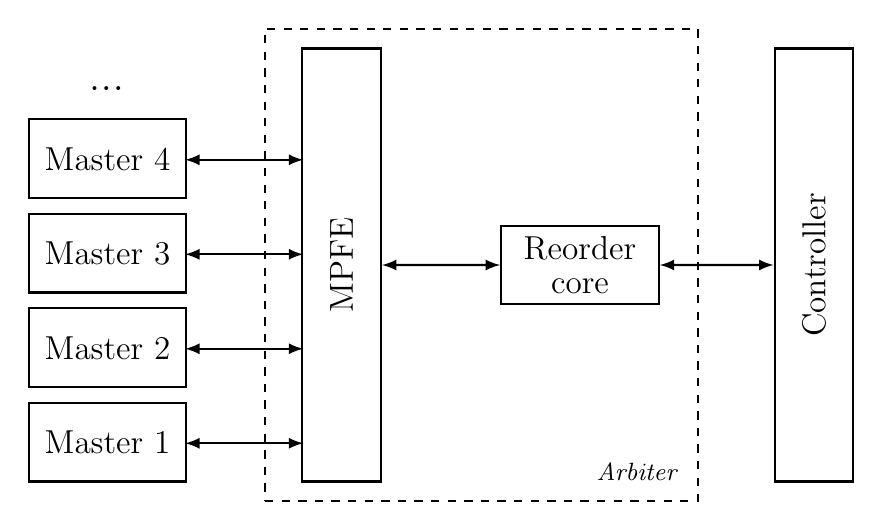
\begin{tikzpicture}[font={\fontsize{12pt}{12}\selectfont}]
    
\node[rectangle, draw, color=black, thick, anchor=south west, minimum width=2cm, minimum height=1cm, inner sep=0pt] (master1) at (0,0) {Master 1};
\node[rectangle, draw, color=black, thick, anchor=south west, minimum width=2cm, minimum height=1cm, inner sep=0pt] (master2) at (0,1.2) {Master 2};
\node[rectangle, draw, color=black, thick, anchor=south west, minimum width=2cm, minimum height=1cm, inner sep=0pt] (master3) at (0,2.4) {Master 3};
\node[rectangle, draw, color=black, thick, anchor=south west, minimum width=2cm, minimum height=1cm, inner sep=0pt] (master4) at (0,3.6) {Master 4};

\node[rectangle, draw, color=black, thick, anchor=south west, minimum width=5.5cm, minimum height=1cm, inner sep=0pt, rotate=90] (MPFE) at (4.5,0) {MPFE};

    \node at (1,5) {{\LARGE ...}};


\draw[<->, >=latex, thick] (2,0.5) -- (3.5,0.5) ;
\draw[<->, >=latex, thick] (2,1.7) -- (3.5,1.7) ;
\draw[<->, >=latex, thick] (2,2.9) -- (3.5,2.9) ;
\draw[<->, >=latex, thick] (2,4.1) -- (3.5,4.1) ;

\node[rectangle, draw, color=black, thick, anchor=south west, minimum width=2cm, minimum height=1cm, inner sep=0pt, align=center] (reorder) at (6,2.25) {Reorder\\ core};

\draw[<->, >=latex, thick] (MPFE.south) -- (reorder.west) ;

\node[rectangle, draw, color=black, thick, anchor=south west, minimum width=5.5cm, minimum height=1cm, inner sep=0pt, rotate=90] (controller) at (10.5,0) {Controller};

\draw[<->, >=latex, thick] (reorder.east) -- (controller.north) ;

\node[rectangle, draw, color=black, thick, anchor=south west, minimum width=5.5cm, minimum height=6cm, inner sep=0pt, dashed]  at (3,-0.25) {};

\node[anchor=south west] at (7.1,-0.1) {\textit{\small Arbiter}};

\end{tikzpicture}
}
    \caption{DDR-SDRAM arbiter of the \mppalong}
    \label{fig_execModel_MPPADRAMarbiter}
\end{figure}
\begin{description}
    \item[Overview]
        The DRAM subsystem can be accessed by 8 \emph{masters} able to read and write in DDR through the 8 ports of the \emph{Multi-Port Front-End} (or \emph{MPFE}, Figure~\ref{fig_execModel_MPPADRAMarbiter}). Two ports are dedicated to handle requests from the 4 RMs and the DSUs of the IODDR and the IOETH cluster in the I/O subsystem. Two other ports are reserved for reads and writes from PCIe backend DMAs. The remaining four ports are reserved for the four DMAs of the IODDR.
    \item[Arbitration]
        As depicted in Figure~\ref{fig_execModel_MPPADRAMarbiter}, the DRAM arbiter of the \mppalong is composed of two elements. The \emph{Multi Port Front End} (or \emph{MPFE}) serializes the requests issued by the masters. Each master (or group of masters) is assigned a priority. In case of concurrent requests, the master with the highest priority will be given full access by the MPFE. Competing masters with the same priority will be arbitrated in Round-Robin. In addition, the MPFE features a \emph{starvation counter} that measures the time during which a request has been pending because of higher priority requests. When this counter reaches a pre-defined level, the pending master is given the maximum priority, thus avoiding starvation.

        The second element of the \mppalong's DRAM arbiter is the \emph{Reorder Core}. It receives requests forwarded by the MPFE and stores them in a pool of $N_{req}^{pool}=8$ elements. Then, it applies the following four rules to decide the order in which the requests will be issued to the controller.

        \begin{description}
            \item[Rule 1] Requests from high priority masters go first;
            \item[Rule 2] Requests on active rows have priority on request targeting non-active rows;
            \item[Rule 3] Requests targeting a recently opened page have low priority during $t_{RC}$;
            \item[Rule 4] \emph{RD} requests have priority over \emph{WR} if previous request was a \emph{RD} and vice versa. 
        \end{description}

        Every time a request is issued to the controller, the reorder core accepts a new request from the MPFE and re-computes the order of requests with the same four rules.

        \begin{example}[Reordering of DRAM requests]
            We assume ascending priorities. The following requests are present in the reordering pool:
            \begin{description}
                \item[Req. 1] \emph{RD} of priority 7 to a non-active row in bank 0;
                \item[Req. 2] \emph{WR} of priority 4 to an active row in bank 1;
                \item[Req. 3] \emph{RD} of priority 4 to a non-active row in bank 0;
                \item[Req. 4] \emph{RD} of priority 4 to a non-active row in bank 1;
                \item[Req. 5] \emph{WR} of priority 7 to an active row in bank 2;
                \item[Req. 6] \emph{WR} of priority 7 to a non-active row in bank 1;
                \item[Req. 7] \emph{WR} of priority 4 to an active row in bank 3;
            \end{description}

            Assuming the four rules of the reorder core, the requests will be served in the following order:
            \begin{description}
                \item[Req. 5] wins Rule 1 with Req. 1 and Req. 6 and wins Rule 2;
                \item[Req. 6] wins Rule 1 with Req. 1 and wins Rule 4;
                \item[Req. 1] wins Rule 1;
                \item[Req. 7] wins Rule 2 (row of Req. 2 has been closed by Req. 6);
                \item[Req. 3] wins Rule 3 (bank 0 is the least recently opened);
                \item[Req. 4] wins Rule 4;
                \item[Req. 2] last request.
            \end{description}
        \end{example}
\end{description}


We will provide further information on the architecture of DRAM subsystems and the methods that have been applied to used them in a predictable manner in Section~\ref{sssec_stateOfTheArt_basicsDRAM}.


\subsection{On-chip networks}
The \mppalong features two parallel NoCs implementing the same 2D-torus topology shown in Figure~\ref{fig_execModel_MPPANoCtopology}. The \emph{Data-NoC} (or \emph{DNoC}) is dedicated for the exchange of large data. The \emph{Control-NoC} or \emph{CNoC} is used to send small control messages to achieve inter-cluster synchronization for example. Both NoCs are wormhole-switched, source-routed, 32 bits wide and running at 600MHz by default.

\subsubsection{Switches}

All the NoC switches are identical (Figure~\ref{fig_execModel_MPPANoCswitch}). The switches have 5 interfaces: North, South, East, West and Local. Each interface has four buffers to store packets received by any of the four other interfaces. In case some flows are conflicting to access an output interface, they are arbitrated in Round-Robin at packet level. Since output buffers are not shared, two flows crossing a switch without interface conflicts will not interfere.
\begin{figure}
    \centering
    \scalebox{0.5}{
% #1 x, #2 y, #3 no
\newcommand\nocswitchbuffer[3]{
    \draw (#1, #2) node[draw, thick, minimum width=1cm, minimum height=0.2cm, anchor=south west, inner sep=0pt] (buf1#3) {};
    \draw (#1, #2 + 0.2) node[draw, thick, minimum width=1cm, minimum height=0.2cm, anchor=south west, inner sep=0pt] (buf2#3) {};
    \draw (#1, #2 + 0.4) node[draw, thick, minimum width=1cm, minimum height=0.2cm, anchor=south west, inner sep=0pt] (buf3#3) {};
    \draw[thick] (#1 + 0.015, #2) -- (#1 + 0.015, #2 - 0.3 );
    \draw[thick] (#1 + 1.015, #2) -- (#1 + 1.015, #2 - 0.3 );
}

% #1 x, #2 y, #3 no
\newcommand\nocswitchint[3]{
    % Draw Round-Robin arbiter
    \draw (#1+ 1.72, #2+ 1.6) node[draw, circle, thick, minimum size = 1cm] (arbiter#3) {};
    \draw[ultra thick, ->, >=latex] (arbiter#3.west) -- ([yshift=-0.6em]arbiter#3.west); 

    % Draw the three buffers
    \nocswitchbuffer{#1}{#2}{n1#3}
    \nocswitchbuffer{#1 + 1.2}{#2}{n2#3}
    \nocswitchbuffer{#1 + 2.4}{#2}{n3#3}

    % Connect the buffers and the arbiter
    \draw[thick, ->, >=latex] (buf3n1#3.north) -- (arbiter#3); 
    \draw[thick, ->, >=latex] (buf3n2#3.north) -- (arbiter#3); 
    \draw[thick, ->, >=latex] (buf3n3#3.north) -- (arbiter#3); 

    % Rx interface
    \draw (#1 - 0.5, #2 - 0.1) node[draw, circle, fill=black, minimum size = 0.3cm, inner sep=0pt] (rx#3) {};

    % Rx and Tx links
    \draw[thick, ->, >=latex] (arbiter#3.north) -- ([yshift=1.5em]arbiter#3.north); 
    \draw[thick, ->, >=latex] ([yshift=7em]rx#3.north) -- (rx#3.north); 
}

\begin{tikzpicture}[font={\fontsize{12pt}{12}\selectfont}]
    % First, the 4 interfaces
    % North
    \nocswitchint{0}{1}{N}
    % South 
    \begin{scope}[rotate=180, transform shape]
        \nocswitchint{-2.8}{5.8}{S}
    \end{scope}
    % East
    \begin{scope}[rotate=90, transform shape]
        \nocswitchint{-3.8}{2}{E}
    \end{scope}
    % West
    \begin{scope}[rotate=-90, transform shape]
        \nocswitchint{1}{4.8}{W}
    \end{scope}
    
    % Connect the interfaces
    % South -> *
    \draw[thick, ->, >=latex] (rxS.south) -- (buf1n3W.south);
    \draw[thick, ->, >=latex] (rxS.south) -- (buf1n2N.south);
    \draw[thick, ->, >=latex] (rxS.south) -- (buf1n1E.south);
    % West -> *
    \draw[thick, ->, >=latex] (rxW.south) -- (buf1n3N.south);
    \draw[thick, ->, >=latex] (rxW.south) -- (buf1n2E.south);
    \draw[thick, ->, >=latex] (rxW.south) -- (buf1n1S.south);
    % North -> *
    \draw[thick, ->, >=latex] (rxN.south) -- (buf1n3E.south);
    \draw[thick, ->, >=latex] (rxN.south) -- (buf1n2S.south);
    \draw[thick, ->, >=latex] (rxN.south) -- (buf1n1W.south);
    % East -> *
    \draw[thick, ->, >=latex] (rxE.south) -- (buf1n3S.south);
    \draw[thick, ->, >=latex] (rxE.south) -- (buf1n2W.south);
    \draw[thick, ->, >=latex] (rxE.south) -- (buf1n1N.south);
    
    % Interface labels
    \node at (0.6,4.5) [text width=2cm, anchor=north, align=center] {{\LARGE North}};
    \node at (2.2,-8.5) [text width=2cm, anchor=north, align=center] {{\LARGE South}};
    \node at (-5,-2.8) [text width=2cm, anchor=north, align=center] {{\LARGE West}};
    \node at (7.7,-1.2) [text width=2cm, anchor=north, align=center] {{\LARGE East}};
\end{tikzpicture}
}
    \caption{NoC switch of the \mppalong. The local interface is not depicted for clarity.}
    \label{fig_execModel_MPPANoCswitch}
\end{figure}

\subsubsection{Routing}
The route that will be followed by a packet is fully defined by software prior to emission. The default header of a DNoC packet includes 43-bits field to store a route. It contains a concatenation of directions encoded on two bits 
(\verb#0x0# to go North, \verb#0x1# to go South, \verb#0x2# to go East, \verb#0x3# to go West) starting from LSB. 

The final destination node of the packet is encoded into the route. The packet reaches the final node when the next direction that it should take is the direction from which it entered the switch. For example, a packet arriving from the east interface is considered as arrived at destination if its next direction is east.

\begin{example}[Routes on the \mppalong]
    A packet following the route: 
    \begin{center}
    \verb#0x2DA = 0b1011011010# 
    \end{center}
    goes east, east, south, west and gets delivered.
\end{example}

The NoC also implements additional features to handle multicast (the packet is delivered to \emph{some} of the nodes on its route) and broadcast (the packet is delivered to \emph{all} nodes on its route) modes. Packet headers can also be extended to account for routes not fitting into 43 bits, up to 104 bits.


\subsection{Remote memory operations}
In this section, we provide further details about the \emph{remote memory operations} on the \mppalong. A \emph{remote write} corresponds to the process of writing data into the memory (either local or external) of a remote cluster. Symmetrically, a \emph{remote read} corresponds to the process of reading data from a distant cluster. We provide two examples of remote reads and writes targeting the external DDR3-SDRAM memory as shown in Figure~\ref{systemModel_MPPAremoteMem}. One may note that remote reads and writes targeting local SRAM of a remote cluster can be achieved with similar processes.


\begin{figure}
\begin{center}
    \begin{picture}(440,275)
		\put(0,0){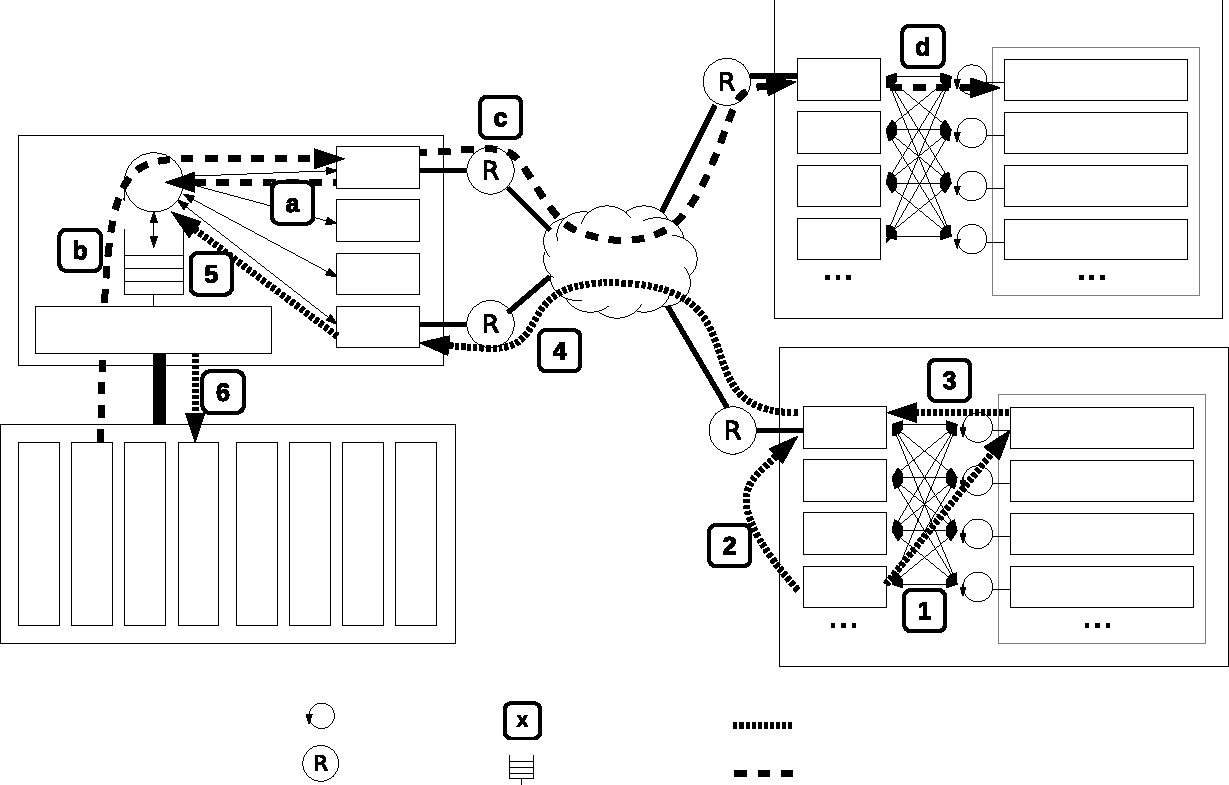
\includegraphics[width=15cm]{imgs/pdf/systemModel_MPPAremoteMem.pdf}}
		\put(371,65){\scriptsize Bank 4}
		\put(371,83){\scriptsize Bank 3}
		\put(371,102){\scriptsize Bank 2}
		\put(371,120){\scriptsize Bank 1}
		\put(368,186){\scriptsize Bank 4}
		\put(368,204){\scriptsize Bank 3}
		\put(368,223){\scriptsize Bank 2}
		\put(368,241){\scriptsize Bank 1}
		\put(350,140){\footnotesize Internal SRAM}
		\put(350,260){\footnotesize Internal SRAM}
		\put(429,146){\rotatebox{270}{\footnotesize Cluster B}}
		\put(427,267){\rotatebox{270}{\footnotesize Cluster A}}
		\put(282,65){\scriptsize Core 3}
		\put(282,83){\scriptsize Core 2}
		\put(282,102){\scriptsize Core 1}
		\put(284,120){\scriptsize DMA}
		\put(279,186){\scriptsize Core 3}
		\put(279,204){\scriptsize Core 2}
		\put(279,223){\scriptsize Core 1}
		\put(282,241){\scriptsize DMA}
		\put(206,179){\footnotesize NoC}
		\put(119,211){\scriptsize DMA 1}
		\put(120,193){\scriptsize Core 2}
		\put(120,175){\scriptsize Core 1}
		\put(119,156){\scriptsize DMA 2}
		\put(23,155){\footnotesize DDR Controller}
		\put(95,127){\footnotesize DDR SDRAM}
		\put(100,227){\footnotesize I/O Cluster}
		\put(10,75){\rotatebox{90}{\scriptsize Bank 1}}
		\put(30,75){\rotatebox{90}{\scriptsize Bank 2}}
		\put(48,75){\rotatebox{90}{\scriptsize Bank 3}}
		\put(66,75){\rotatebox{90}{\scriptsize Bank 4}}
		\put(86,75){\rotatebox{90}{\scriptsize Bank 5}}
		\put(104,75){\rotatebox{90}{\scriptsize Bank 6}}
		\put(123,75){\rotatebox{90}{\scriptsize Bank 7}}
		\put(141,75){\rotatebox{90}{\scriptsize Bank 8}}
		\put(122,21){\footnotesize Arbiter}
		\put(122,5){\footnotesize NoC Router}
		\put(194,20){\footnotesize Process step}
		\put(194,5){\footnotesize Queue}
		\put(282,18){\footnotesize Write process}
		\put(282,4){\footnotesize Read process}
	\end{picture}

	\caption{Example of remote memory operations on a simplified model of the \mppalong}
	\label{systemModel_MPPAremoteMem}
\end{center}
\end{figure}

\begin{example}[Remote write]
In this example, the core 3 of cluster B requires to write data in the bank 4 of the external DDR3-SDRAM memory. We detail each step of this write process as shown in figure~\ref{systemModel_MPPAremoteMem} 
    (the \emph{Write process} is numbered with \emph{numbers} and depicted with dotted arrows in figure~\ref{systemModel_MPPAremoteMem}):
\begin{enumerate}
    \item[1.] The requesting computing core (core 3 of cluster B) writes the data to be sent in the local memory of the compute cluster. As the banks of the local SRAM are shared among many potential requesters, there may be an arbitration at this level in the case of concurrent accesses to the bank. 
	\item[2.] The core signals to the local DMA its intention to send the data.
	\item[3.] DMA reads the data (written by core 3 at step 1) from the local memory. Once again, any concurrent access to the same bank will involve an arbitration.
	\item[4.] DMA sends the data through the NoC. If the amount of data to send is important, it will be split in several packets constituting a flow. All the packets will cross the NoC following the same path. If one or several parts of this NoC path are shared with other NoC flows, the arbitration between the flows will occur at packet level.
	\item[5.] The sink DMA (DMA 2 of the I/O cluster) receives the packets and initiates DDR3-SDRAM write transactions. If other masters (I/O cores, other DMAs, \ldots) access the external memory concurrently, an arbitration process will occur. This phase assumes that the sink DMA has been configured before reception to associate one of its reception queues to a specific DDR3-SDRAM address (an address in bank 4 of the DDR3-SDRAM here). 
	\item[6.] Once the sink DMA write(s) request(s) is/are elected by the memory arbiter, data is written into the DDR3-SDRAM array.
\end{enumerate}
\end{example}


\begin{example}[Remote read]
    In this example, the core 2 of cluster A needs to read data from the bank 2 of the DDR-SDRAM to store it in the bank 1 of its local memory. We detail each step of this read process as shown in figure~\ref{systemModel_MPPAremoteMem} (the \emph{Read process} is numbered with \emph{letters} and dashed arrows in figure~\ref{systemModel_MPPAremoteMem}):

\begin{enumerate}
    \item[a.] The DMA of the I/O cluster initiates a DDR3-SDRAM read transaction. Once again, any concurrent access to the memory with any other master will involve arbitration.
    \item[b.] Once the DMA command is elected, data is transferred from DDR3-SDRAM to the DMA.
    \item[c.] DMA sends packets through the NoC. Again, important amounts of data are packetized and arbitrated with concurrent flows at packet level.
    \item[d.] DMA of the compute cluster receives the packets and attempts to write them back into the local memory. Again, we assume that this DMA has been pre-configured to associate one of its reception queue to a specific memory area of the local memory (the bank 1 in this example). 
\end{enumerate}

    We remark that a read process is fairly equivalent to a write process. Indeed, a read by a computing core is equivalent to a write from an IO cluster. The difference is that the destination of the data is not the external memory but the internal memory of a Compute cluster.

    In this example, the phase \emph{a.} of the read process is initiated by the DMA of the I/O cluster. It is assumed here that the DMA is either responding to a read request that was previously sent by the requesting cluster or started automatically following a scheduling table computed off-line.
\end{example}





\subsection{Compatibility with a safety-critical context}
The \mppalong can be considered as a good COTS target candidate for the design of hard-real time systems for several reasons listed below. 

\begin{description}
    \item[Low energy consumption]
    Although saving power is obviously beneficial to reduce fuel consumption in an aircraft, it also greatly helps the design of certifiable electronics cards. Indeed, it appears that, under specific conditions, the power consumption of the \mppalong is probably sufficiently low to cool with purely passive systems. Being able to avoid active cooling dramatically simplifies the design of electronics cards that are robust to vibrations constraints.

    \item[Timing-compositionality]
    The k1b cores exhibit the property of \emph{full timing-compositionality}, that, as we will further explain in Section~\ref{sec_stateOfTheArt_WCETestimation}, greatly simplifies the computation of the safe WCETs required for certification.

    \item[High programmability]
    On the \mppalong, very few operations are achieved implicitly - the hardware does not support cache coherency and messages are sent on the NoC explicitly. Although this specificity does not simplify programming, it does help in mastering the platform with software. In addition, NoC communications are heavily configurable using custom DMA micro-codes and the source routing mechanism. So, many different communication patterns can be implemented in a very flexible but still controlled way.

    \item[Information availability]
    The willingness of \kalray to share extensive information regarding their architecture's details with clients is a significant asset from an industrial point of view. Indeed, as we will further explain in Section~\ref{sec_stateOfTheArt_WCETestimation}, the common industrial practice of computing WCET using \emph{static analysis} requires fine-grained models of the platform. Being able to obtain the informations to construct these models is thus of major importance.
\end{description}



\section{Additional constraints}
\label{sec_systemModel_additionalConstraints}
%\subsection{Industrial constraints}
In an industrial environment, two criteria are of particular interest: cost and performance. Designing inexpensive avionics systems usually implies strong design constraints on the choice of hardware components, 
on the architecture of systems, and on the certification of software. 
As an example, current industrial practices privilege COTS over bespoke hardware components in many situations for both cost and performance reasons. Designing and producing \emph{powerful} custom-made processors requires important investments. In contrary, choosing COTS can dramatically reduce hardware design costs and narrow the design lead time overall. As a consequence, we will focus in this thesis on the challenges for designing software managing the caveats of a COTS platform such as the \mppalong. The architecture and implementation of such software are detailed in Chapters~\ref{chap_execModel} and~\ref{chap_implemExecMod}. 

\begin{constraint}
    \label{constr_cotsOnly}
    COTS processors must be used for performance.
\end{constraint}


In safety critical systems, and in particular in avionics, industrial standards, such as the DO-178C~\cite{do178}, impose the computation of safe upper-bounds on the \emph{Worst-Case Execution Time} (or \emph{WCET}) of software programs. Computing such bounds can be challenging~\cite{Wilhelm2008} because execution times vary depending on input parameters and current hardware states. Moreover, the WCET estimation problem is becoming increasingly harder with the emergence of multi and many-core processors~\cite{Wilhelm2012}. This is due to more complex internal behaviours, shared resources and interferences. The challenge is thus twofold: 1) since modern architecture are particularly complex to analyze, producing \emph{safe} WCET estimations appears especially difficult; and 2) WCET estimations must be \emph{tight} to avoid too much resource over-provisioning that eventually leads to poor performance. In this context, the major constraint is to design systems that can be analyzed in order to \emph{make WCET computation feasible}. In Chapter~\ref{chap_boundingExecTimes}, we will overview the classical methods to estimate WCET on modern multi- and many-core platforms and how systems can be designed in order to be make their analysis practically doable.

\begin{constraint}
    \label{constr_staticAnalysis}
    Computing WCET of program using static analysis techniques must be practically feasible.
\end{constraint}




Industrial practices imply that off-line scheduling is often preferred to on-line scheduling when dealing with safety-critical applications. The reason for this is twofold. Firstly, the execution of off-line scheduled tasks can be achieved using simple scheduling tables. Since this requires a minimal run-time support, the certification cost of the system software can be kept low. And secondly, mapping tasks off-line simplifies the overall timing analysis of the system by avoid context-switching costs or preemption-related overheads. For this reason, we will focus in this thesis on the problems related to the off-line scheduling of safety-critical application only. We propose in Chapter~\ref{chap_budgetValidation} an off-line approach for mapping hard-time applications on the \mppalong.

\begin{constraint}
    \label{constr_schedOffLine}
    Scheduling of tasks must be achieved off-line.
\end{constraint}

Finally, modern avionics applications are massive. Managing such applications requires approaches not only providing good results on small examples but also on industrial-sized problem instances. For this reason, our goal in this thesis will be not only to find solutions to the different problems related to mapping and scheduling but also to find solutions having a direct practical interest to solve current industrial problems. Consequently we will evaluate the scalability of the mapping technique detailed in Chapter~\ref{chap_budgetValidation} over a real avionics application from Airbus.

\begin{constraint}
    \label{constr_scalability}
    All mapping and scheduling techniques must scale to industrial-sized applications.
\end{constraint}

%Finally, real avionics applications are large. Managing such applications requires approaches not only providing good results on small examples but also on industrial-sized problem instances. For this reason, our goal in this thesis will be not only to find solutions to the different problems related to mapping and scheduling but also to find solutions having a direct practical interest to solve current industrial problems. Consequently we will  evaluate the scalability of the mapping technique detailed in Chapter~\ref{chap_budgetValidation} against a real avionics application from Airbus.




\section{Summary}
In this chapter, we have detailed the context of the thesis, its consequences on the input data of the various programming and scheduling problems to be solved, as well as the methods that can be envisaged to do so. We consider real avionics applications modeled by multi-rate parallel tasks with explicit data exchanges. Our goal will be to execute these applications on the \mppalong that can arguably be considered as a good candidate for the design of future avionics computers.
The industrial context will limit our investigations to off-line mapping techniques in order to have better control of the target and to keep the certification costs as low as possible. Finally, since we aim at solving industrial problems, we will have a major requirement regarding the scalability of our solutions in order to deal with applications of realistic sizes as shown in Chapter~\ref{chap_budgetValidation}.



\clearpage
\subbiblio

\end{document}



